\section{Conversión de numero Binario a Decimal}

\subsection{Descripción del problema}
Este programa tiene como objetivo dado un numero binario de n bits regresar su equivalente en decimal.

\begin {figure}[h!]
\centerline{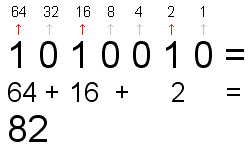
\includegraphics[width = 4cm]{Latex-imágenes/binario.png}}
\caption{Binario a decimal.}
\label{fig}
\end {figure}


\subsection{Definición  de solución}
Para poder hacer la conversión es necesario ingresar un numero binario. Basta con numerar los dígitos de derecha a izquierda comenzando desde cero, a cada número se le asigna la correspondiente potencia base 2 y al final se suman las potencias\cite{articuloBinario} 

\begin {figure}[h!]
\centerline{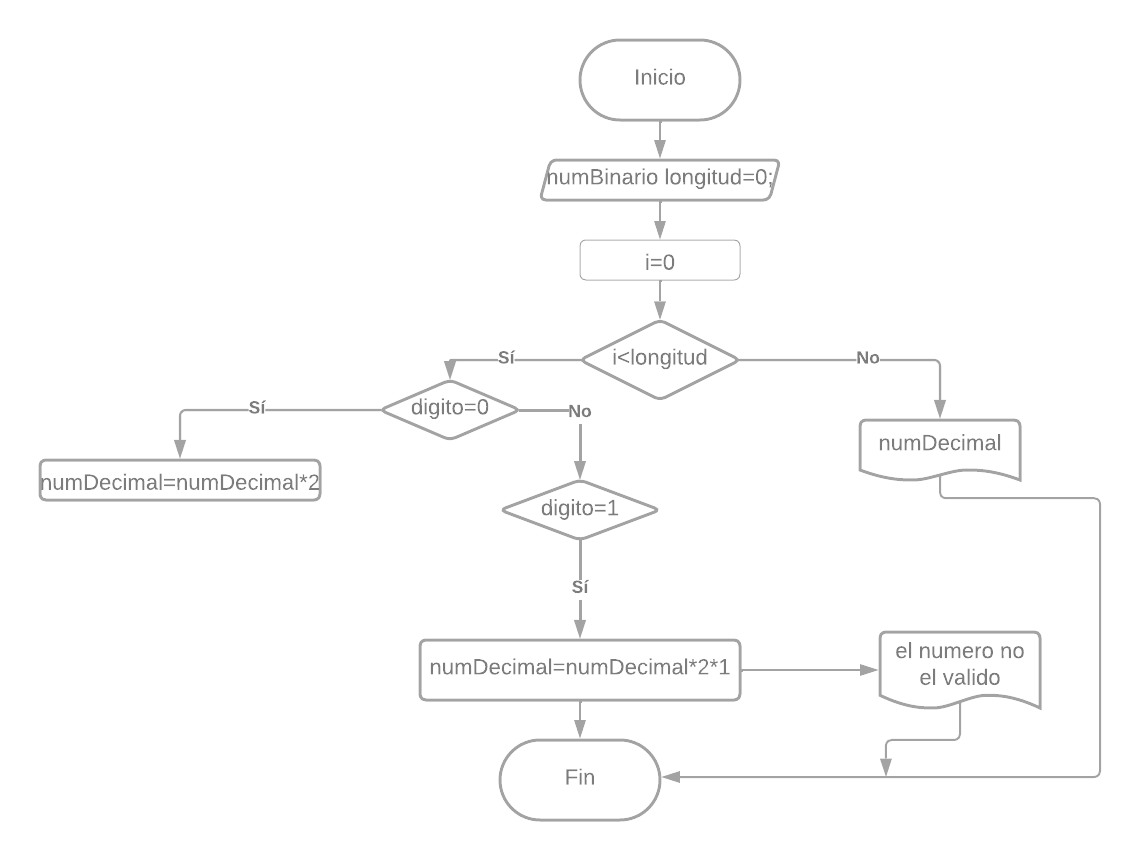
\includegraphics[width = 6cm]{Latex-imágenes/Diagramaejercicio5.png}}
\caption{Binario a decimal.}
\label{fig}
\end {figure}



\subsection{Diseño de Solución}

\begin{enumerate}
  \item El programa comienza pidiendo que se ingrese un numero binario
  \item luego el programa calcula la longitud del numero binario
  \item Se inicia un bucle for que recorre cada dígito del número binario
  \item En cada iteración del bucle, se obtiene el dígito actual utilizando el método charAt(i) y se almacena en la variable digito
  \item Se verifica si el dígito es '0'. Si es así, se multiplica numeroDecimal por 2 sin agregar ningún valor adicional
  \item Si el dígito es '1', se multiplica numeroDecimal por 2 y se le suma 1
  \item Si el dígito no es ni '0' ni '1', se muestra en la consola el mensaje "El numero binario ingresado no es valido"
  \item Después de recorrer todos los dígitos del número binario, se muestra en la consola el resultado de la conversión
  
\end{enumerate}


% En este apartado va el codigo del problea
\subsection{Desarrollo de Solución}
El diseño del programa sigue la estructura y se implementa la .
\begin{javaCode}
int longitud = numeroBinario.length();
        int numeroDecimal = 0;
        for (int i = 0; i < longitud; i++) {
            char digito = numeroBinario.charAt(i);
            //Verificar si es 0 o 1
            if (digito == '0') {
                numeroDecimal = numeroDecimal * 2;
            } else if (digito == '1') {
                numeroDecimal = numeroDecimal * 2 + 1;
            } else {
                System.out.println("El numero binario ingresado no es valido");
                return;
            }
        }
        System.out.println("El numero decimal equivalente es:" + numeroDecimal);
    }
}
\end{javaCode}


%En este apartado va la corrida del ejercicio
\subsection{Depuración y pruebas}
 \begin{tabular}{|c|c|c|}
  \hline
  numCorrida & binario & conversión \\
  \hline
  1 & 101& 5 \\
  \hline
  2 & 0111 & 7 \\
  \hline
  3 & d24 & valor no valido \\
  \hline
\end{tabular}

